\section{Filtro notch pasivo}

Se conoce como filtro notch o rechaza banda a la configuración de circuito electrico que "elimina" las señales cuyas frecuencias son cercanas a la frecuencia de corte del filtro, dejando pasar en el resto de las frecuencias.

A partir de los resultados obtenidos de la parte grupal del trabajo práctico, se realiza un análisis de la respuesta en frecuencia del circuito planteado y el diseño del circuito en un PCB.

\subsection{Cálculo, simulación y medición}

Se mantiene el mismo circuito analizado en la parte grupal, con la diferencia que ahora los componentes adoptan los siguientes valores:

\begin{itemize}[leftmargin=2cm]
	\item $R_1 = R_2 = 3.3K\Omega$
	\item $R_3 = 1.5K\Omega$
	\item $C_1 = C_2 = 18nF$
	\item $C_3 = 39nF$
  \end{itemize}

\begin{figure}[h]
	\centering
	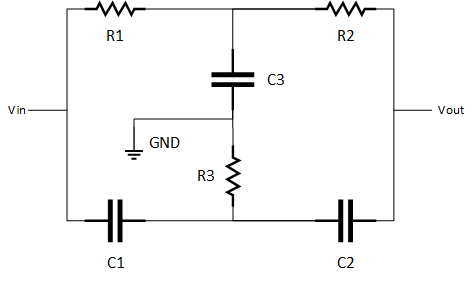
\includegraphics[scale=1]{../Informe/Imagenes/circuito.png}
	\caption{Filtro Notch Pasivo}
	\label{ej1cir}
\end{figure}

Debido a que aproximadamente $C_1 = C_2 = 2C_3$ y con un margen un poco mayor $R_1 = R_2 = 2R_3$, se decide emplear la función transferencia obtenida del TP grupal para el análisis:

$$\hspace{0.5cm} H(s) = \frac{s^2C^2R^2 + 1}{s^2R^2C^2 + s4RC + 1}$$

Ya que en el circuito para $R_1$ y $R_2$ se usó el valor comercial de resistencias de $3.3k\Omega$, se emplea ese valor junto a $C = 18nF$ en la función transferencia. Reemplazando, se obtiene la función:

$$\hspace{0.5cm} H(s) = \frac{3.53\cdot 10^{-9}\cdot s^{2} + 1}{3.53\cdot 10^{-9}\cdot s^{2} + 2.38\cdot 10^{-4}\cdot s + 1}$$

Obteniendo una frecuencia de corte igual a:
$$f_0 = \frac{1}{2\pi RC} \Rightarrow \hspace{0.5cm} f_0 \approx 2679.38 Hz$$.

A fin de estudiar la respuesta en frecuencia del circuito, se realizó una simulación en LTSpice estableciendo los parametros para un análisis de Monte Carlo.

\begin{figure}[h]
	\centering
	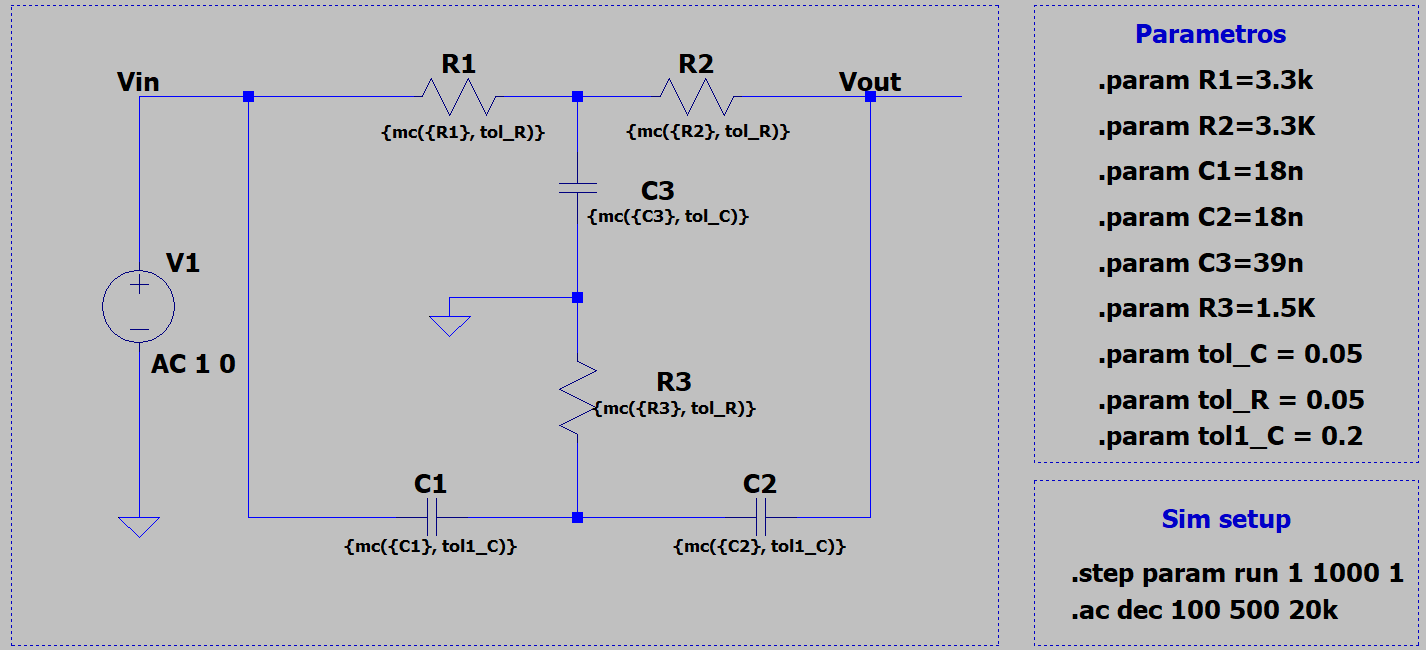
\includegraphics[scale=0.4]{../Informe/Imagenes/simu.png}
	\caption{Simulación en LTSpice}
	\label{ej1cir}
\end{figure}

Asimismo, se estudió el circuito usando componentes comerciales con el equipo $Digilent$ $electronics$ $explorer$, provisto por la universidad, obteniendo mediciones mediante la plataforma $WaveForms$.

Para realizar el circuito, se utilizaron resistores comerciales del valor planteado con una tolerancia del $5\%$; un capacitor de $39nF$ con una tolerancia nomninal del $20\%$; dos capacitores de $100nF$ y dos de $22nF$, ambos con tolerancia del $5\%$, dispuestos en serie para obtener una capacitancia aproximada de $18.033nF$, valor sumamente cercano a los requeridos.

En la construcción del circuito en el protoboard se trató de minimizar el uso de cables entre los componentes para evitar sumar resistencias adicionales, aunque mínimas. 

\begin{figure}[H]
	\centering
	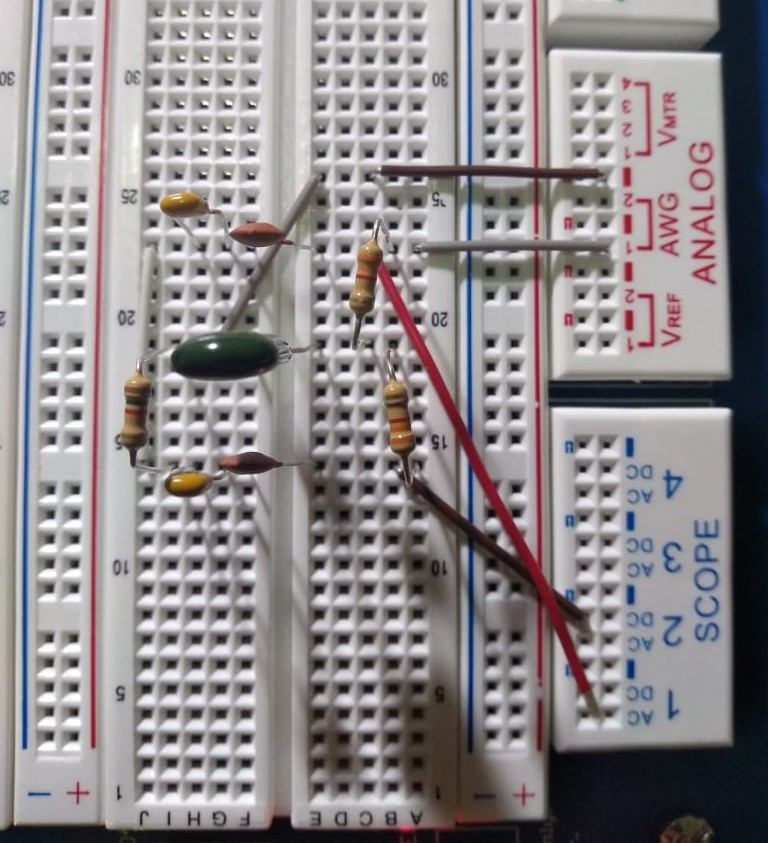
\includegraphics[scale=0.4]{../Informe/Imagenes/NotchProto.jpeg}
	\caption{Circuito en protoboard}
\end{figure}

\subsection{Diseño de PCB}

Para poder medir realmente el circuito en funcionamiento en la práctica, se requeriría imprimirlo en PCB, conectar sus componentes, alimentarlo con una fuente y relevar los valores con un osciloscópio. 

Se diseñó un prototipo del circuito planteado. Se dispusieron pistas de 0,7 mm, con chanfles a 45°. 

\begin{figure}[H]
	\centering
	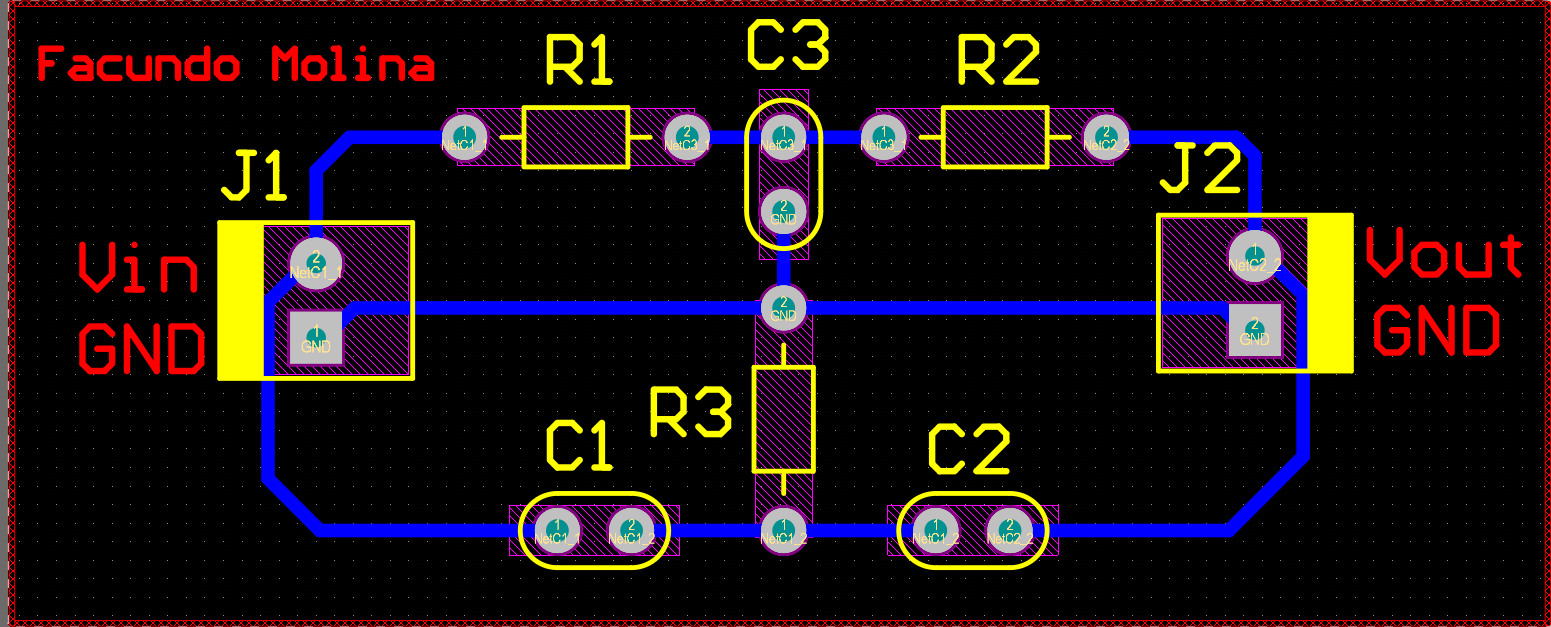
\includegraphics[scale=0.4]{../Informe/Imagenes/PCB.png}
	\caption{Diseño de PCB en Altium}
\end{figure}


\subsection{Análisis de resultados}

Se construyeron las funciones transferencia en escala semilogarítmica a partir de la función teórica, la simulación en LTSpice y de las mediciones relevadas en $WaveForms$. Se las superpuso de modo de realizar un análisis. Del Monte Carlo en LTSpice se representaron 14 mediciones.

\begin{figure}[H]
\centering
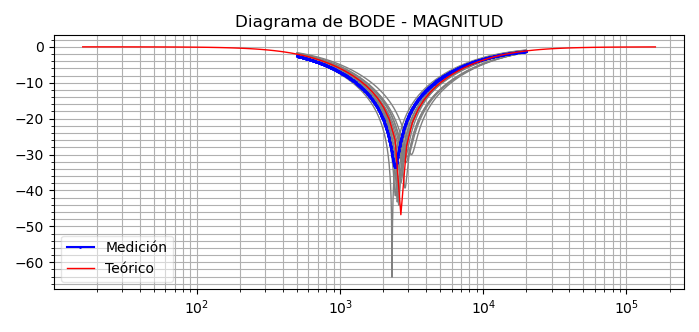
\includegraphics[scale =1]{../Informe/Imagenes/Ej1Gain2.png}
\caption{Diagrama de Bode: Ganancia. Superposición ganancia teórica, medida y simulada (gris)}
\end{figure}

\begin{figure}[H]
	\centering
	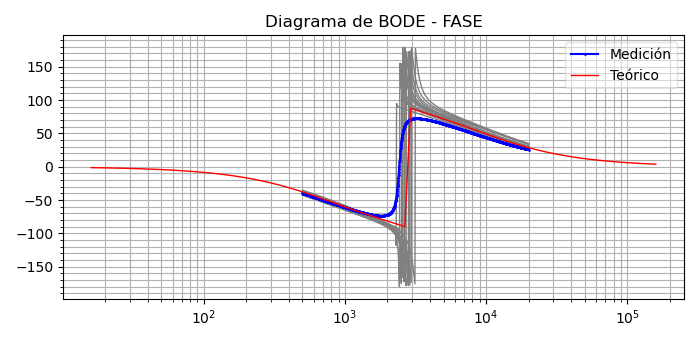
\includegraphics{../Informe/Imageness/Ej1Phase2.png}
	\caption{Diagrama de Bode: Fase. Superposición fase teórica, medida y simulada (gris)}
\end{figure}


Como mayores características de la función transferencia del filtro notch, resalta la pronunciada caída en la ganancia alrededor de la frencuencia de corte y el salto en la fase al pasar por dicho valor. 
Aunque con discrepancias, se visualiza una similitud entre las curvas, aproximándo en la práctica a los valores esperados teoricamente. No obstante, se puede notar que el mínimo de la ganancia medida es menor a lo esperado por la teoría en la frecuencia de corte. Esto último se podría deber a la dificultad que se tiene en medir la señal cuando esta tiene una frecuencia cercana a la de corte y por la diferencia de los valores nominales y reales de los componentes. Por otra parte, los gráficos discrepan en cuanto al valor de la frecuencia de corte teórica, siendo menor en el gráfico de las mediciones. Esto último se puede deber al hecho que para estudiar la función teórica en este informe se empleó una aproximación junto a que los componentes pueden presentar una variación. Aun así, se visualiza que los resultados teóricos y medidos se encuentran dentro de los simulados mediante el Monte Carlo en LTSpice, el cual permite analizar la respuesta del circuito teniendo en cuenta las tolerancias mencionadas de los componentes utilizados.

En cuanto a la fase, el salto en las mediciones y simulación se da en un intervalo y no de forma inmediata como lo que se preveía teoricamente, hecho que se debe a que en la realidad el cambio no es inmediato. 


